% ============================================================================
% Report — Image-quality inductive bias for MedVAE (Théophile's part)
%
% MERGE NOTE: content intended to replace \section{Section 2:
% Théophile} (empty) in final.tex, between section IV (JEPA) and
% section VI (Segmentation). The master document already loads:
% graphicx, amsmath/amssymb, booktabs, cite, balance, float, dblfloatfix,
% subcaption.
%
% Copy the figures/theophile/ folder next to final.tex (at the same level
% as figures/elias/, figures/yanic/, figures/theo/) before pasting the
% content below (between BEGIN/END SECTION) into final.tex.
%
% This file also compiles standalone (preamble below, to be removed at
% merge time) for preview purposes.
% ============================================================================
\documentclass[conference]{IEEEtran}
\usepackage[utf8]{inputenc}
\usepackage[T1]{fontenc}
\usepackage{graphicx}
\usepackage{amsmath,amssymb}
\usepackage{booktabs}
\usepackage{cite}
\usepackage{balance}
\usepackage{float}
\usepackage{dblfloatfix}
\usepackage{subcaption}
\usepackage{placeins}

\begin{document}
\pagestyle{plain}

% ============================================================
% BEGIN SECTION — to be pasted in place of \section{Section 2: Théophile}
% ============================================================
\section{Image-quality inductive bias for MedVAE}
\label{sec:theophile}

\subsection{Motivation}

The previous section showed that MedVAE behaves as an intelligent low-pass
filter and a non-linear denoiser, but that it has no explicit way of
knowing \emph{how much} the image it is given is degraded: it applies the
same transformation to a clean or a heavily noisy angiography. Yet this
information is available \emph{a priori} and can be estimated by
no-reference quality metrics (NR-IQA). We hypothesise that explicitly
conditioning the autoencoder on a quality score $c \in [0,1]$ improves its
reconstruction, by letting it adapt its behaviour to the degradation level
actually present at the input. Three questions follow: how to compute $c$
objectively and reproducibly in the absence of human annotation on
ARCADE; how to inject it into MedVAE without retraining the model from
scratch; and whether any observed gain is attributable to the informative
content of $c$ or to a mere additional-capacity effect. This last
question is far from trivial: any conditioning mechanism adds parameters
and changes the training dynamics, so an apparent gain could simply
reflect increased capacity rather than a genuine exploitation of the
quality signal, hence the need for a dedicated ablation
(section~\ref{sec:ablation}). For the first question, three independent
methods for computing $c$ (approaches A, B, C) are compared in parallel,
and the entire downstream pipeline (conditioning, training, evaluation,
ablation) is run separately for each, which makes it possible to
distinguish an effect specific to a given method of computing $c$ from a
more general effect of the FiLM conditioning itself.

\subsection{Construction of the quality score}
\label{sec:score}

On the segmentation subset of ARCADE (1000 train / 200 validation images,
$512\times512$, grayscale), each image is split into a $4\times4$ grid of
patches, a local granularity motivated by the spatially non-uniform
nature of artefacts in cardiac imaging (motion, noise)
\cite{sekiguchi2025patchdsa}, normalised by \emph{Mean Subtracted Contrast
Normalization} ($\hat{I}=(I-\mu)/(\sigma+C)$, $7\times7$ window), then
characterised by 8 metrics per patch: Laplacian variance, RMS contrast,
Shannon entropy, and the Tenengrad gradient broken down into 4
directions, a directional analysis suited to the tubular structure of
vessels \cite{wang2024noreference} (which allows detection of anisotropic
cardiac motion blur). These metrics are aggregated into 36 features per
image. A pre-trained ResNet-18 (frozen weights) extracts in parallel a
512-dimensional feature vector, used only by the learned approach: the
two branches of this feature pipeline (Figure~\ref{fig:featpipe}) never
converge directly, they simply feed different score-computation methods
(section~\ref{sec:score}).

\begin{figure}[t]
  \centering
  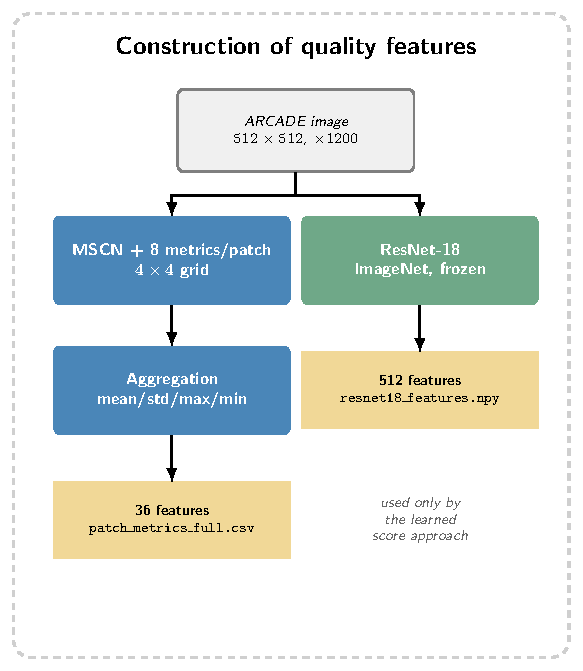
\includegraphics[width=0.85\columnwidth]{pipeline_A_features.pdf}
  \caption{Construction of quality features: per-patch IQA metrics and
  ResNet-18 features.}
  \label{fig:featpipe}
\end{figure}

These features are then merged into a single score $c$, with $1$
corresponding to a clinically usable image, using three independent
methods (Figure~\ref{fig:scorepipe}), all fitted exclusively on the TRAIN
subset. Approach B applies a PCA (after standardisation) on 6 selected
features (the 36 above plus two spatial-homogeneity and directional-balance
features); the first axis explains 56.1\,\% of the variance, and its sign
is corrected by correlation with Tenengrad ($r=0.952$). Approach A
linearly weights the same 6 features by the absolute normalised loadings
of this same PC1. Approach C, lacking human annotation on ARCADE, learns
a score on a \emph{synthetic proxy}, an indirect supervision strategy
already used to calibrate NR-IQA scores on biomedical images without
perceptual ground truth \cite{asri2026deeplearning}: each TRAIN image is
artificially degraded (noise, blur, JPEG) with a target
$y=1-\text{known severity}$, and a lightweight MLP
($512{\to}128{\to}32{\to}1$) is trained by MSE on the ResNet-18 features of
this synthetic set (validation MSE $1.58\times10^{-3}$), then applied to
the real images.

\begin{figure*}[t]
  \centering
  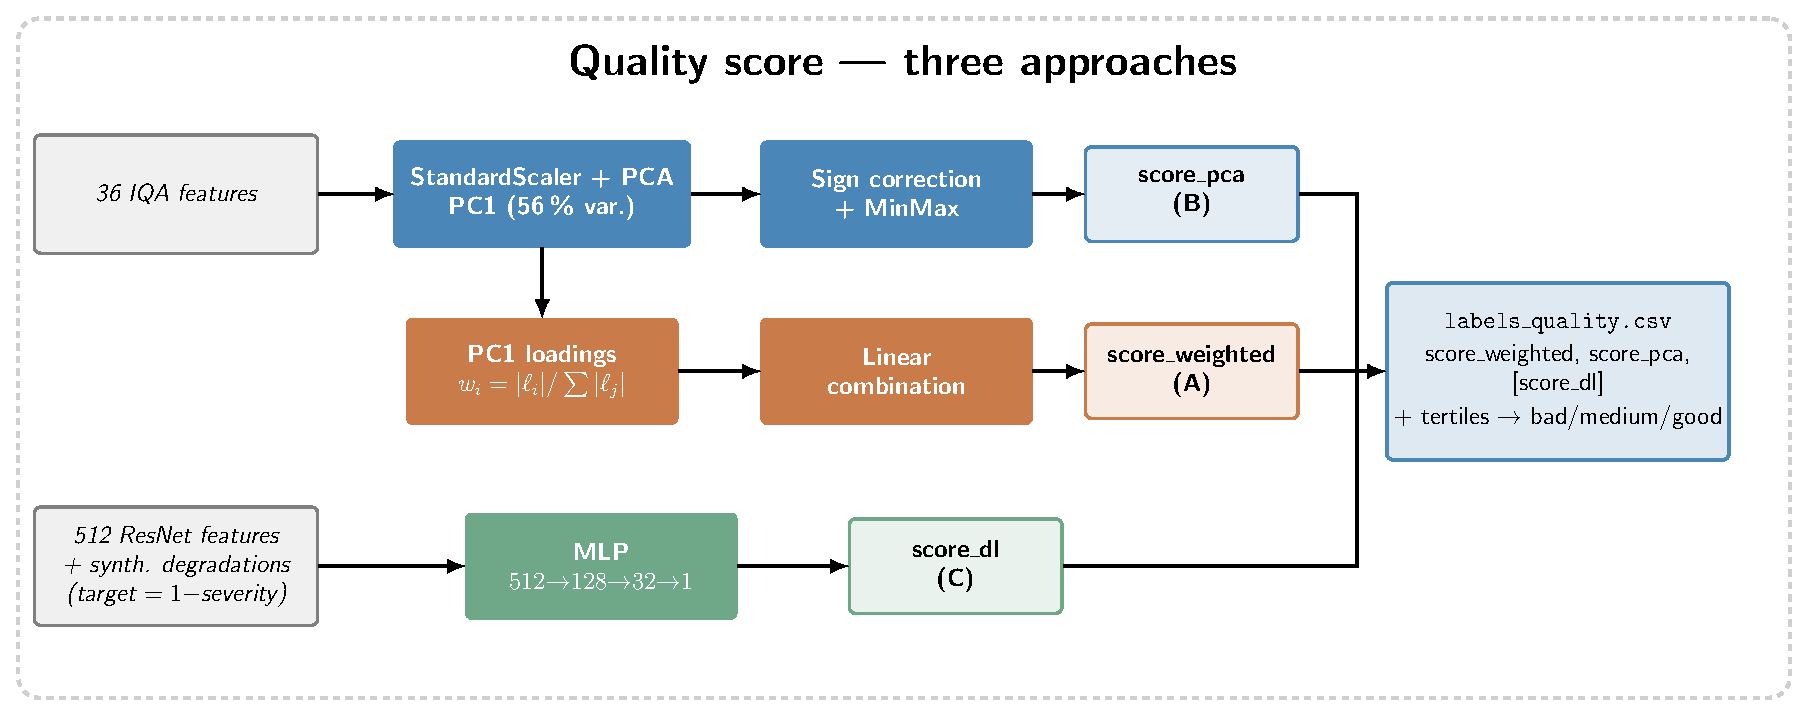
\includegraphics[width=0.92\textwidth]{pipeline_B_score.pdf}
  \caption{The three approaches for computing the quality score $c$.}
  \label{fig:scorepipe}
\end{figure*}

A and B, built on the same metrics, are strongly correlated ($r=0.884$);
C, in contrast, is nearly independent of both
($r(A,C)=0.003$, $r(B,C)=0.015$, Table~\ref{tab:corr}) and its
distribution is much more tightly concentrated near 1 (mean 0.890) than A
(0.448) or B (0.483): the MLP learned on deep features captures a notion
of quality that differs from a combination of classical metrics. The
active score is finally discretised into three classes
\emph{bad}/\emph{medium}/\emph{good} by tertiles (TRAIN). Figure~\ref{fig:gallery}
illustrates this progression on real images sorted by increasing score:
the least sharp and noisiest angiographies (left) progressively give way
to contrasted acquisitions where the vascular tree is clearly defined
(right), which qualitatively confirms that the score captures a notion of
image quality consistent with a clinical reading.

\begin{figure}[t]
  \centering
  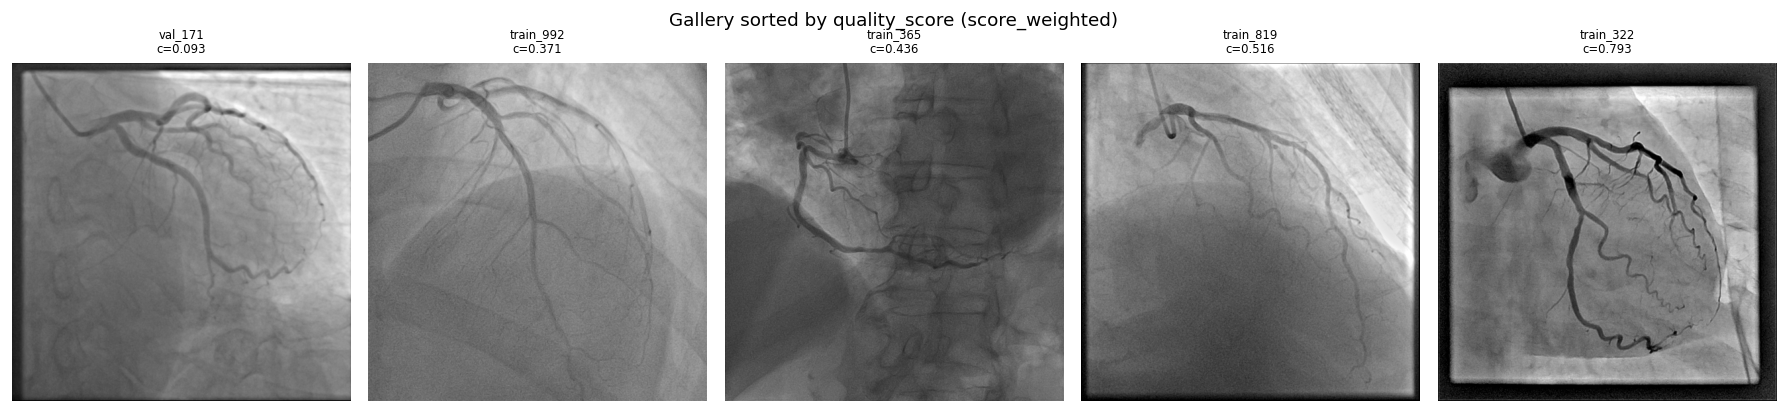
\includegraphics[width=\columnwidth]{result_gallery_score.png}
  \caption{ARCADE images sorted by increasing quality score (approach A,
  weighted): from least sharp (left) to most contrasted (right).}
  \label{fig:gallery}
\end{figure}

\begin{table}[htbp]
  \centering
  \begin{tabular}{@{}lccc@{}}
    \toprule
     & A (weighted) & B (PCA) & C (learned) \\
    \midrule
    A (weighted) & 1 & 0.884 & 0.003 \\
    B (PCA)      &   & 1     & 0.015 \\
    C (learned)  &   &       & 1 \\
    \bottomrule
  \end{tabular}
  \caption{Pearson correlation between the three scores (1200 images).}
  \label{tab:corr}
\end{table}

\FloatBarrier
\subsection{FiLM conditioning and training}
\label{sec:film}

To condition MedVAE \cite{varma2025medvae} (pre-trained
\texttt{AutoencoderKL} \cite{kingma2014autoencoding}, variant
\texttt{medvae\_4\_1\_2d}, 57.06M parameters) on $c$ without modifying its
input topology, we use \emph{Feature-wise Linear Modulation}
(FiLM \cite{perez2018film}) rather than channel concatenation: a shared
MLP encodes $c$ into a 128-dimensional embedding, and 19 linear heads (one
per \texttt{ResnetBlock} of the encoder, bottleneck, and decoder) produce
affine parameters applied through a hook on each block,
$h \leftarrow (1+\gamma_i(c)) \cdot h + \beta_i(c)$, with zero
initialisation (the conditioned model is therefore identical to the
original model before any training). This initialisation choice matters:
it guarantees that any performance difference observed after training
stems from what the network has learned to do with $c$, and not from a
random perturbation of the pre-trained weights. FiLM is further preferred
over input-channel concatenation because it leaves the encoder's topology
intact and concentrates the conditioning effect on clearly identifiable
parameters, which facilitates the ablation in
section~\ref{sec:ablation}. This mechanism adds 1.70M parameters
(2.98\,\%). Training proceeds in two phases on the 1000 TRAIN images
resized to $64\times64$: a warm-up where only FiLM is trained (2500
steps, low learning rate) to avoid destabilising the pre-trained decoder
with still poorly calibrated affine parameters, then a global fine-tuning
where all weights are unfrozen (5000 steps, cosine annealing) to let the
rest of the network adapt to the FiLM modulation. A strictly identical
baseline VAE without FiLM is trained in parallel on the same budget of
7500 steps, in order to isolate the conditioning's own effect from that of
additional fine-tuning (Figure~\ref{fig:filmpipe}).

\begin{figure*}[t]
  \centering
  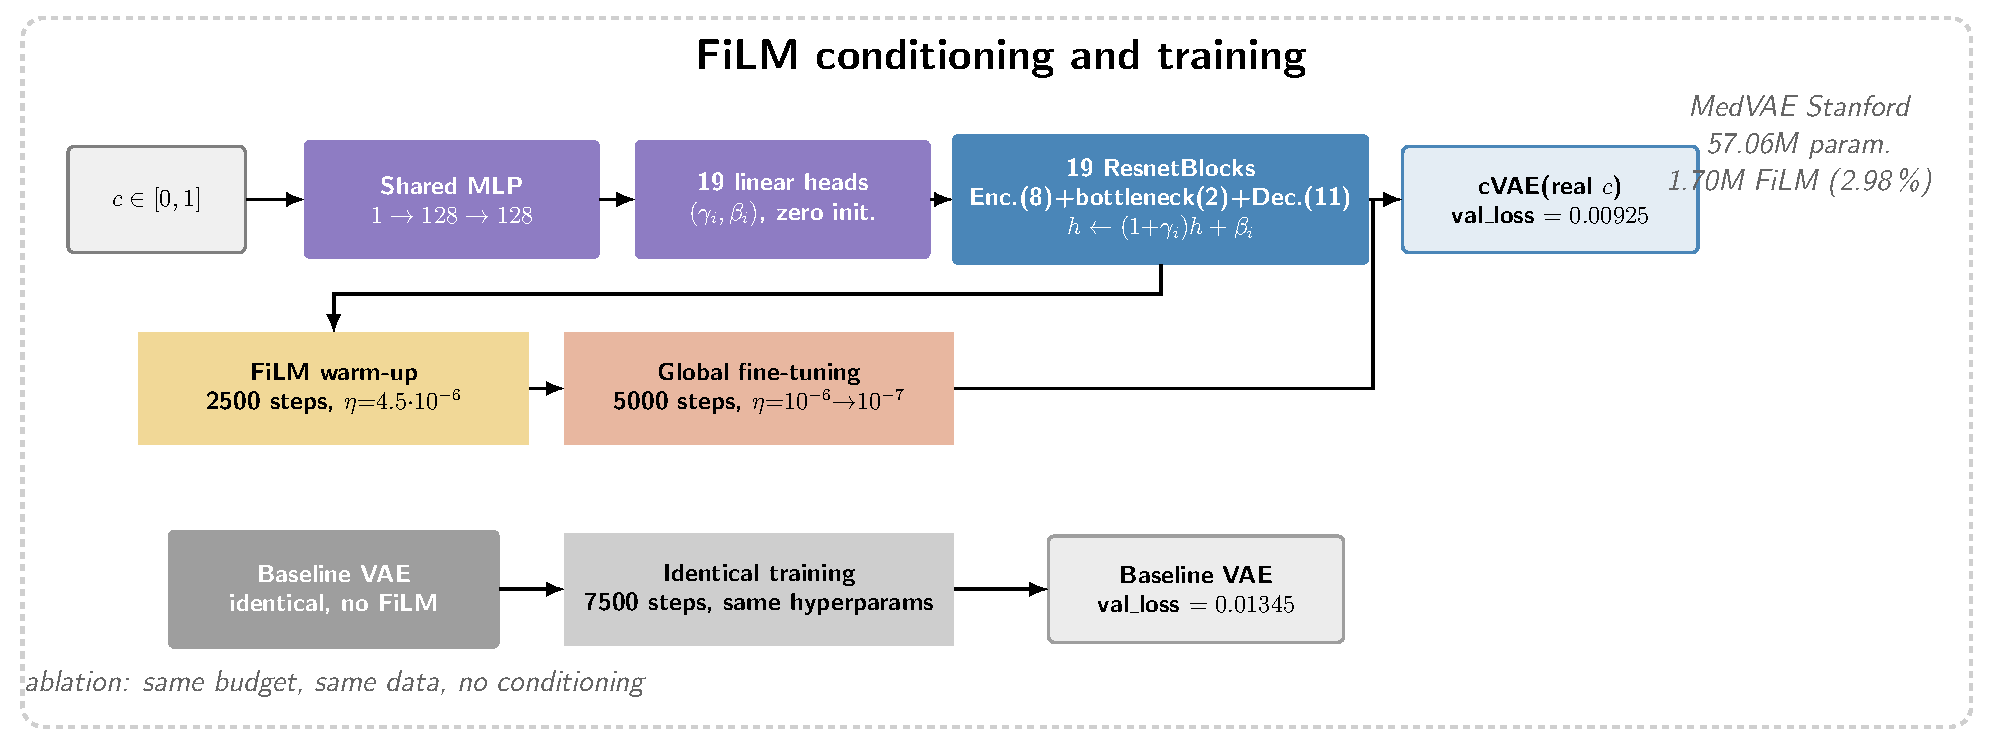
\includegraphics[width=0.92\textwidth]{pipeline_C_film.pdf}
  \caption{FiLM conditioning (19 blocks) and two-phase training, with
  baseline ablation.}
  \label{fig:filmpipe}
\end{figure*}

\begin{table}[htbp]
  \centering
  \begin{tabular}{@{}lccc@{}}
    \toprule
    Approach & cVAE($c$) & Baseline & Relative gain \\
    \midrule
    A (weighted) & 0.00735 & 0.01345 & $-45.3\%$ \\
    B (PCA)      & 0.00749 & 0.01348 & $-44.5\%$ \\
    C (learned)  & 0.00925 & 0.01345 & $-31.2\%$ \\
    \bottomrule
  \end{tabular}
  \caption{Final validation ELBO loss ($64\times64$, internal to
  training), conditioned cVAE vs baseline, per approach.}
  \label{tab:trainloss}
\end{table}

On this internal loss, the conditioned cVAE is markedly better than the
baseline for all three approaches (Table~\ref{tab:trainloss}), a result
that seems to validate the initial hypothesis, but which only measures
optimisation on the reduced fine-tuning format, not reconstruction
fidelity on independent test images at full resolution.

\FloatBarrier
\subsection{Evaluation of reconstruction fidelity}
\label{sec:eval}

On a test set of 60 images (20 per class, unseen during training), we
compare the reconstruction of the cVAE and the baseline using four
metrics (MSE, SSIM, PSNR, HaarPSI, the latter being recommended for
medical images \cite{breger2024adequacy}), both on the full image and on
a masked PSNR restricted to vessel pixels (mPSNR, rasterised COCO
annotations). This restriction makes it possible to check that any
observed result is not a mere artefact of the background, clinically
irrelevant and potentially misleading since a global PSNR can
\emph{increase} as the image degrades
% TODO merge: replace with \ref{...} to the MedVAE robustness section
(cf. the MedVAE robustness analysis presented earlier)
(Figure~\ref{fig:evalpipe}).

\begin{figure}[t]
  \centering
  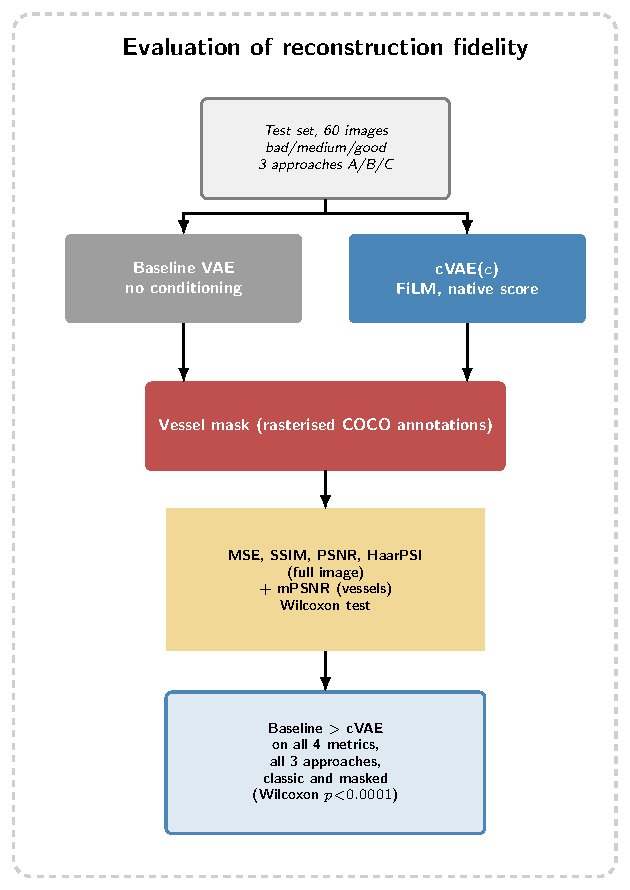
\includegraphics[width=0.82\columnwidth]{pipeline_D_evaluation.pdf}
  \caption{Evaluation protocol: baseline vs cVAE, classic and masked
  (vessel) PSNR.}
  \label{fig:evalpipe}
\end{figure}

\begin{table}[htbp]
  \centering
  \begin{tabular}{@{}lcccc@{}}
    \toprule
    Approach & MSE & SSIM & PSNR & HaarPSI \\
    \midrule
    A (weighted) & $+21.1\%$ & $-1.6\%$ & $-2.4\%$ & $-1.6\%$ \\
    B (PCA)      & $+26.1\%$ & $-1.7\%$ & $-2.7\%$ & $-1.9\%$ \\
    C (learned)  & $+48.8\%$ & $-1.8\%$ & $-4.4\%$ & $-2.1\%$ \\
    \bottomrule
  \end{tabular}
  \caption{Relative change of cVAE vs baseline (60 real images; MSE:
  positive = worse; others: negative = worse). All differences are
  significant (Wilcoxon $p<0.0001$).}
  \label{tab:eval}
\end{table}

The result runs counter to the initial hypothesis: across all three
approaches and all four metrics, without exception, the unconditioned
baseline reconstructs better than the cVAE (Table~\ref{tab:eval}), and
this does not change when restricting the error to vessels: mPSNR confirms
the same ranking for all three approaches, with a systematic gap of $2$ to
$5$~dB relative to classic PSNR (vessels, thin and low-contrast, remain
intrinsically harder to reconstruct than the background,
% TODO merge: replace with \ref{...} to the MedVAE robustness section
consistent with the MedVAE robustness analysis presented earlier). The
per-class breakdown (Table~\ref{tab:mpsnr-class}) confirms that this
baseline $>$ cVAE ranking is uniform across all 9
approach$\times$class combinations (bad/medium/good), without a single
exception, and is confirmed under controlled synthetic degradations
(noise, motion blur): the baseline matches or exceeds the cVAE on almost
all levels tested. The internal validation loss
(Table~\ref{tab:trainloss}), more favourable to the cVAE, therefore turns
out to be a misleading indicator of actual performance.

\begin{table}[htbp]
  \centering
  \footnotesize
  \begin{tabular}{@{}lcccccc@{}}
    \toprule
    & \multicolumn{2}{c}{A (weighted)} & \multicolumn{2}{c}{B (PCA)} & \multicolumn{2}{c}{C (learned)} \\
    Class & base & cVAE & base & cVAE & base & cVAE \\
    \midrule
    bad    & 31.42 & 29.96 & 32.07 & 30.55 & 30.57 & 29.42 \\
    medium & 30.62 & 29.72 & 31.33 & 29.57 & 30.87 & 29.34 \\
    good   & 30.97 & 29.89 & 29.72 & 28.48 & 31.37 & 29.75 \\
    \bottomrule
  \end{tabular}
  \caption{mPSNR (dB), baseline vs cVAE, per approach and quality class
  (60 test images). The baseline wins on all 9 combinations, without a
  single exception.}
  \label{tab:mpsnr-class}
\end{table}

This regularity also holds within each class: the dispersion of the
baseline/cVAE gap remains comparable between the two models across all
three metrics, so this is not an effect driven by a few outlier images,
but a systematic shift of the entire distribution.

\FloatBarrier
\subsection{Ablation with a constant signal}
\label{sec:ablation}

The previous result calls for checking whether the network nonetheless
exploits the informative content of $c$, even without deriving a net
gain from it. A second cVAE is trained with exactly the same
architecture, the same data, and the same budget, but presenting a
constant $c=0.5$ for all images; at inference, both models receive the
true score of each test image, and only the value \emph{seen during
training} differs between the two (Figure~\ref{fig:ablationpipe}).

\begin{figure}[t]
  \centering
  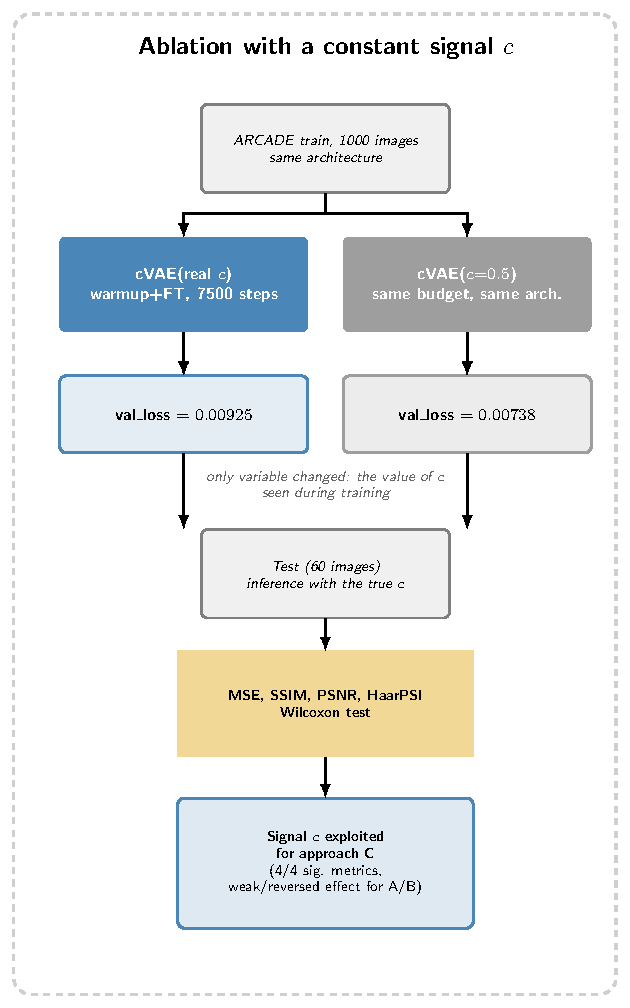
\includegraphics[width=0.78\columnwidth]{pipeline_E_ablation.pdf}
  \caption{Ablation with a constant signal $c$: same architecture, same
  data, only the supervision of $c$ changes.}
  \label{fig:ablationpipe}
\end{figure}

\begin{table}[htbp]
  \centering
  \begin{tabular}{@{}lccc@{}}
    \toprule
     & real $c$ wins & $c{=}0.5$ wins & Not sig. \\
    \midrule
    A (weighted) & 0/4 & 2/4 & 2/4 \\
    B (PCA)      & 2/4 & 0/4 & 2/4 \\
    C (learned)  & 4/4 & 0/4 & 0/4 \\
    \bottomrule
  \end{tabular}
  \caption{Number of metrics (out of 4) where cVAE(real $c$) significantly
  beats cVAE($c{=}0.5$) (Wilcoxon $p<0.05$, 60 images).}
  \label{tab:ablation}
\end{table}

This more nuanced result depends strongly on the approach
(Table~\ref{tab:ablation}): only C unambiguously demonstrates that signal
$c$ is exploited, on all four metrics ($p<10^{-4}$), a finding also
confirmed by mPSNR across all three classes without exception. For B, the
effect is partial (MSE and PSNR significant, not SSIM/HaarPSI), and the
per-class mPSNR shows verdict reversals depending on the metric. For A,
the effect is even reversed on two perceptual metrics: a constant
$c=0.5$ performs better than the true weighted score.

Figure~\ref{fig:delta} details, for approach C, the per-image gap between
cVAE(real $c$) and cVAE($c{=}0.5$) as a function of the tested image's
quality score: the advantage of real conditioning grows with $c$, and
reverses slightly for the most degraded images (\emph{bad}), where a
constant $c=0.5$, close to the median, acts almost as a reasonable default
signal. The network has therefore indeed learned a response that
\emph{depends} on $c$, and not merely a response to the presence of a
non-zero embedding.

\begin{figure}[t]
  \centering
  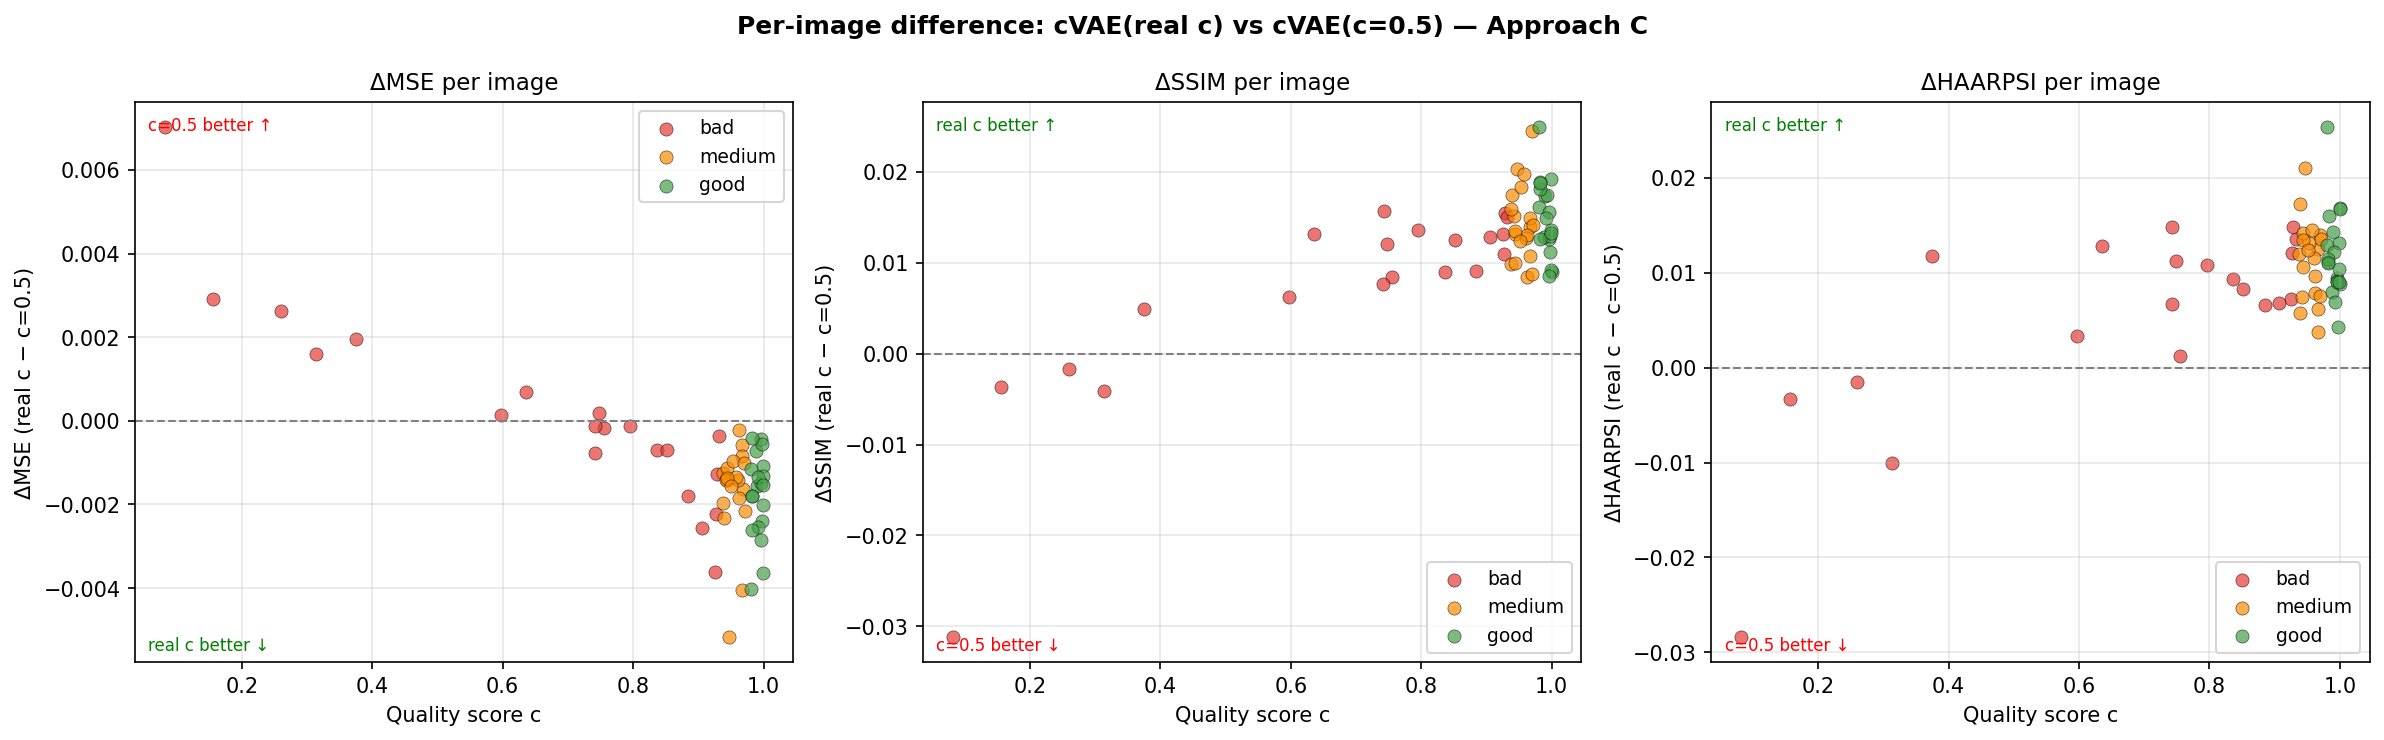
\includegraphics[width=\columnwidth]{result_delta_ablation.png}
  \caption{Per-image gap (MSE, SSIM, HaarPSI) between cVAE(real $c$) and
  cVAE($c{=}0.5$) as a function of the quality score, approach C.}
  \label{fig:delta}
\end{figure}

\FloatBarrier
\subsection{Discussion}
\label{sec:discussion-theophile}

Taken together, these experiments tell a richer story than a simple
validation of the initial hypothesis. FiLM conditioning, correctly
measured on an independent test set and in pixel space, slightly degrades
reconstruction fidelity relative to an unconditioned VAE trained with the
same budget. This result is robust, significant across three approaches
and four metrics, and survives the restriction to vessel pixels. The
ablation nuances this negative finding: for approach C, the network
unambiguously exploits the informative content of $c$, so the observed
degradation is not due to inert conditioning, but rather to a genuine
architectural trade-off, where the additional FiLM capacity and per-layer
modulation appear to perturb the decoder's optimisation more than they
enrich it, within the budget used. For A and B, the effect of $c$ is
weaker or even reversed, suggesting that their scores, linear combinations
of sharpness and contrast metrics, provide information already largely
accessible to the network through its own convolutions.

The near-independence between score C and scores A/B
(Table~\ref{tab:corr}, $r\approx0$) calls for caution when interpreting
the learned score: trained on a synthetic severity proxy rather than a
human ground truth, it could encode a signal partially different from
true perceptual quality. That this signal is exploited by the network
without nonetheless improving reconstruction is consistent with this
reading: the network learns \emph{something} useful from $c_C$, but not
necessarily a better reconstruction strategy.

Several limitations of this protocol deserve mention. First, the training
budget (7500 steps, $64\times64$ resolution) remains modest relative to
the size of MedVAE (57M parameters): an architectural FiLM trade-off that
penalises the decoder at this stage could lessen, or even reverse, with a
longer budget or a more gradual warm-up. Second, the absence of human
quality annotation on ARCADE forced us to validate the three scores
indirectly (mutual consistency, correlation with reference metrics)
rather than against a perceptual ground truth; a study with clinicians
would help determine whether the learned score (C), the only one truly
exploited by the network, captures a clinically meaningful notion of
quality or an artefact of the synthetic proxy used to supervise it.
Finally, the criterion used here (pixel/structural fidelity) does not
directly measure downstream clinical utility (e.g. readability of the
vascular tree for diagnosis); future work could couple this protocol to a
segmentation or detection task to check whether FiLM conditioning, even
if slightly unfavourable for raw reconstruction, does not bring a benefit
on a task-oriented metric.

% --------------------------------------------------------------------------
% MERGE NOTE: these references are specific to this part. They need to be
% merged manually with final.tex's shared bibliography (which already
% lists MedVAE and Kingma & Welling under other keys): deduplicate
% varma2025medvae/kingma2014autoencoding against the existing entries and
% renumber the \cite commands accordingly.
% --------------------------------------------------------------------------
\begin{thebibliography}{99}

\bibitem{perez2018film}
E.~Perez, F.~Strub, H.~de Vries, V.~Dumoulin, and A.~Courville,
``FiLM: Visual reasoning with a general conditioning layer,'' in
\emph{Proc. AAAI Conf. on Artificial Intelligence}, 2018.

\bibitem{breger2024adequacy}
A.~Breger \emph{et al.}, ``A study on the adequacy of common IQA measures
for medical images,'' \emph{arXiv:2405.19224}, 2024.

\bibitem{wang2024noreference}
Z.~Wang, S.~Chen, J.~Dai, S.~Qin, Y.~Cao, R.~Zhao, G.~Wu, Y.~Tang, and
J.~Chen, ``A no-reference medical image quality assessment method based on
automated distortion recognition technology: application to preprocessing
in MRI-guided radiotherapy,'' \emph{arXiv:2412.06599}, 2024.

\bibitem{asri2026deeplearning}
M.~A.~A.~Asri, H.~Rajagopal, N.~Mokhtar, W.~A.~W.~M.~Mahiyiddin,
Y.~A.~L.~Lim, M.~Iwahashi, R.~Harakawa, F.~Ibrahim, and T.~Ito,
``Deep learning-based no-reference image quality assessment framework for
\emph{Cryptosporidium} spp. and \emph{Giardia} spp.,'' \emph{PLOS ONE},
2026.

\bibitem{sekiguchi2025patchdsa}
Y.~Sekiguchi, T.~Okamoto, T.~Matsuzawa, K.~Fujimoto, K.~Fujiwara,
T.~Kondo, J.~Koizumi, and H.~Haneishi, ``PatchDSA: improving digital
subtraction angiography with patch-based phase-matching in natural
breathing scenarios,'' \emph{Radiological Physics and Technology}, vol.~18,
no.~3, pp.~698--706, 2025.

\bibitem{varma2025medvae}
M.~Varma, A.~Kumar, R.~van der Sluijs, S.~Ostmeier, L.~Blankemeier,
P.~Chambon, C.~Bluethgen, J.~Prince, C.~Langlotz, and A.~Chaudhari,
``MedVAE: efficient automated interpretation of medical images with
large-scale generalizable autoencoders,'' \emph{arXiv:2502.14753}, 2025.

\bibitem{kingma2014autoencoding}
D.~P.~Kingma and M.~Welling, ``Auto-encoding variational Bayes,'' in
\emph{Proc. Int. Conf. on Learning Representations (ICLR)}, 2014.

\end{thebibliography}

% ============================================================
% END SECTION
% ============================================================

\end{document}
